\documentclass[twocolumn, 12pt]{article}

\usepackage[utf8]{inputenc}
\usepackage[english, spanish]{babel}
\usepackage[papersize={216mm,330mm},tmargin=15mm,bmargin=15mm,lmargin=15mm,rmargin=15mm]{geometry}
\usepackage{fullpage}
\usepackage{graphicx}
\usepackage{amsmath}
\usepackage{enumitem}
\usepackage{chngcntr}
\usepackage{setspace}
\usepackage{url}
\usepackage{csquotes}
\usepackage{float}
\usepackage{verbatim}
\usepackage{tabularx}
\usepackage{amsmath}
\usepackage{caption}

\counterwithin{figure}{section}
\renewcommand{\thesection}{\arabic{section}}
\renewcommand{\thesubsection}{\thesection.\arabic{subsection}}
\renewcommand{\baselinestretch}{1.5}

\usepackage[style=apa, maxnames=6, minnames=3, backend=biber]{biblatex}
\DefineBibliographyStrings{english}{%chktex-file 1 chktex-file 6
    andothers = {\em et\addabbrvspace al\adddot}
}
\addbibresource{./Bibliography/bibliography.bib}

\usepackage{array}
\usepackage{enumitem}
\usepackage{longtable}

\setlength{\parskip}{0pt}

\raggedbottom{}

\begin{document}

\begin{titlepage}
    \centering
    
\includegraphics[width=0.3\textwidth]{Images/logo_utb.png}\par\vspace{1cm}
    {\scshape\LARGE Universidad Tecnológica de Bolívar \par}
    \vspace{1.5cm}

    {\scshape\Large FÍSICA ELÉCTRICA \par}
    \vspace{.2cm}

    % chktex-file 8
    \vspace{2cm}
    % chktex-file 8
    \slshape {\Large \bfseries{} RC CIRCUIT SIMULATION\\}
    \vspace{3cm}

    \slshape {\itshape{} Mauro González, T67622 \\}
    \slshape {\itshape{} German De Armas Castaño, T68765 \\}
    \slshape {\itshape{} Angel Vega Rodriguez, T68186 \\}
    \slshape {\itshape{} Juan Jose Osorio Ariza, T67316 \\}
    \vfill

    Revisado Por \\ David Sierra Porta \\

    {\large \today\par}
\end{titlepage}

~\nocite{GoogleDrive}

% -----------------------------------------------------------|>
\section{Datos experimentales}

\begin{table}[H]
    \captionsetup{justification=centering}
    \centering

    % chktex-file 44
    \begin{tabularx}{0.9\linewidth}{|>{\centering\arraybackslash}X|>{\centering\arraybackslash}X|}
        \hline
        \multicolumn{2}{|c|}{Constantes}              \\ \hline

        $\varepsilon$ \textit{(V)}            & $30$  \\\hline
        Resistencia \textit{($\Omega$)}       & $80$  \\\hline
        Capacitancia \textit{($\mathcal{F}$)} & $0.2$ \\\hline
        RC \textit{($\tau$)} \textit{[Seg]}   & $16$  \\\hline
    \end{tabularx}

\end{table}

\begin{table}[H]
    \centering
    \begin{tabularx}{0.9\linewidth}{|>{\centering\arraybackslash}X|>{\centering\arraybackslash}X|}

        \hline
        \multicolumn{2}{|c|}{Carga}                  \\\hline
        Tiempo \textbf{[Seg]} & Voltaje \textbf{[V]} \\\hline
        $0.0$                 & $0.0$                \\\hline
        $5.5$                 & $9.65$               \\\hline
        $10.4$                & $15.01$              \\\hline
        $15.6$                & $19.15$              \\\hline
        $20.2$                & $21.9$               \\\hline
        $25.4$                & $24.13$              \\\hline
        $30.4$                & $25.73$              \\\hline
        $35.5$                & $26.89$              \\\hline
        $40.3$                & $27.7$               \\\hline
        $45.3$                & $28.31$              \\\hline
        $50.4$                & $28.77$              \\\hline
        $55.5$                & $29.11$              \\\hline
        $60.3$                & $29.34$              \\\hline
        $65.5$                & $29.52$              \\\hline
        $70.3$                & $29.65$              \\\hline
        $75.5$                & $29.75$              \\\hline
        $80.3$                & $29.81$              \\\hline
        $85.6$                & $29.86$              \\\hline
        $90.5$                & $29.9$               \\\hline
        $95.5$                & $29.93$              \\\hline
        $100.4$               & $29.95$              \\\hline

    \end{tabularx}
\end{table}

\begin{figure}[H]
    \centering
    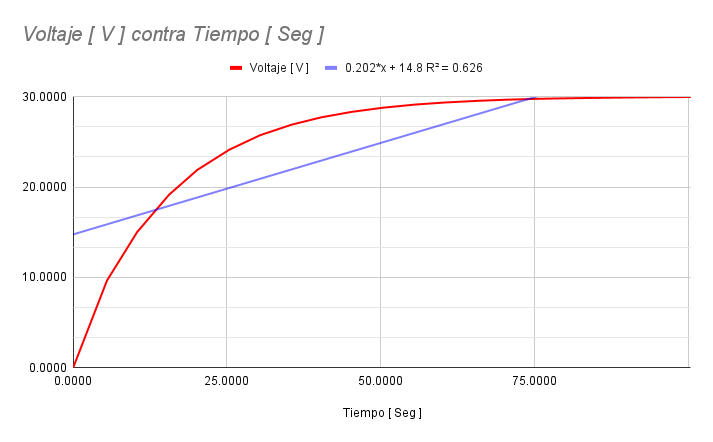
\includegraphics[width=\linewidth]{./Images/Voltaje [ V ] contra Tiempo [ Seg ].png}
\end{figure}

\begin{itemize}[label=$\triangleright$]
    \item Linea de tendencia:\hfill \break{} $0.202 \cdot x + 14.8
              R^2 = 0.626$
\end{itemize}

\begin{table}[H]
    \centering
    \begin{tabularx}{0.9\linewidth}{|>{\centering\arraybackslash}X|>{\centering\arraybackslash}X|}

        \hline
        Tiempo \textbf{[Seg]} & $\ln (1- \frac{V}{\varepsilon})$ \\\hline
        $0.0$                 & $0$                              \\\hline
        $5.5$                 & $-0.3881164698$                  \\\hline
        $10.4$                & $-0.6938140695$                  \\\hline
        $15.6$                & $-1.017032302$                   \\\hline
        $20.2$                & $-1.30933332$                    \\\hline
        $25.4$                & $-1.631342748$                   \\\hline
        $30.4$                & $-1.949583554$                   \\\hline
        $35.5$                & $-2.266574655$                   \\\hline
        $40.3$                & $-2.568288259$                   \\\hline
        $45.3$                & $-2.876468853$                   \\\hline
        $50.4$                & $-3.194183212$                   \\\hline
        $55.5$                & $-3.517731198$                   \\\hline
        $60.3$                & $-3.816712826$                   \\\hline
        $65.5$                & $-4.135166557$                   \\\hline
        $70.3$                & $-4.451019506$                   \\\hline
        $75.5$                & $-4.787491743$                   \\\hline
        $80.3$                & $-5.061928588$                   \\\hline
        $85.6$                & $-5.367310238$                   \\\hline
        $90.5$                & $-5.703782475$                   \\\hline
        $95.5$                & $-6.060457419$                   \\\hline
        $100.4$               & $-6.396929655$                   \\\hline

    \end{tabularx}
\end{table}

\begin{figure}[H]
    \centering
    % chktex-file 36
    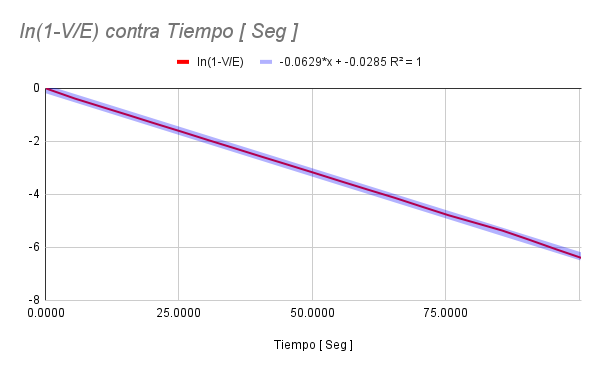
\includegraphics[width=\linewidth]{./Images/ln(1-V_E) contra Tiempo [ Seg ].png}
\end{figure}

\begin{itemize}[label=$\triangleright$]
    \item Linea de tendencia:\hfill \break{} $-0.0629 \cdot x -0.0285
              R^2 = 1$
\end{itemize}

\begin{table}[H]
    \centering
    \begin{tabularx}{0.9\linewidth}{|>{\centering\arraybackslash}X|>{\centering\arraybackslash}X|}

        \hline
        \multicolumn{2}{|c|}{Descarga}               \\\hline
        Tiempo \textbf{[Seg]} & Voltaje \textbf{[V]} \\\hline
        $0.0$                 & $29.99$              \\\hline
        $5.5$                 & $20.82$              \\\hline
        $10.3$                & $15.26$              \\\hline
        $15.5$                & $11.0$               \\\hline
        $20.3$                & $8.17$               \\\hline
        $25.3$                & $5.97$               \\\hline
        $30.3$                & $4.35$               \\\hline
        $35.5$                & $3.14$               \\\hline
        $40.3$                & $2.33$               \\\hline
        $45.4$                & $1.0$                \\\hline
        $50.3$                & $1.24$               \\\hline
        $55.3$                & $0.91$               \\\hline
        $60.3$                & $0.67$               \\\hline
        $65.4$                & $0.49$               \\\hline
        $70.3$                & $0.36$               \\\hline
        $75.2$                & $0.26$               \\\hline
        $80.3$                & $0.19$               \\\hline
        $85.3$                & $0.14$               \\\hline
        $90.6$                & $0.1$                \\\hline
        $95.3$                & $0.07$               \\\hline
        $100.2$               & $0.05$               \\\hline
    \end{tabularx}
\end{table}

\begin{figure}[H]
    \centering
    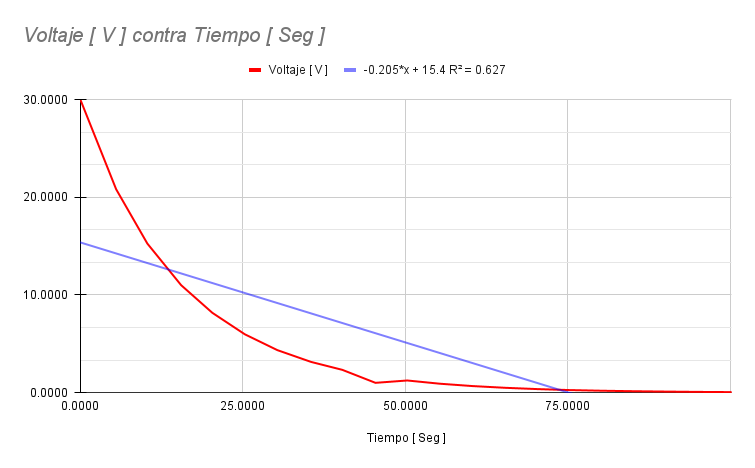
\includegraphics[width=\linewidth]{./Images/Voltaje [ V ] contra Tiempo [ Seg ] Descarga.png}
\end{figure}

\begin{itemize}[label=$\triangleright$]
    \item Linea de tendencia:\hfill \break{} $-0.205 \cdot x + 15.4
              R^2 = 0.627$
\end{itemize}

% -----------------------------------------------------------|>
\section{Charging a capacitor}

% ----------------------------------------|>
\subsection{Using the equations above what is the time constant $\tau$? (Seg)}

Usando la ecuación, $\tau = R \cdot C$, tenemos, $\tau = 80
    \Omega \cdot 0.2 \mathcal{F} = 16 Seg$

% ----------------------------------------|>
\subsection{When t = $\tau$ what is the value of the voltage? (V)}

Usando la ecuación,

{\large
        \begin{equation}
            V_c = \frac{q}{c} = \varepsilon (1 - e^{\frac{-t}{RC}})
            \label{eq:voltaje__Carga}
        \end{equation}
    }

$V_c = 30V (1 - e^{-1}) = 18,9636V$

% ----------------------------------------|>
\subsection{What percentage of the battery voltage is the voltage across the capacitor at this time?}

Usando la ecuación~\eqref{eq:voltaje__Carga} despejada,

{\large
        \begin{equation}
            \frac{V_c}{\varepsilon} = 1 - e^{\frac{-t}{RC}}
            \label{eq:voltaje__Carga-Porcentaje}
        \end{equation}
    }

Si $\tau = RC$, $\frac{V_c}{\varepsilon} = 1 - e^{-1} =
    0.6321\%$

% ----------------------------------------|>
\subsection{When t = $2\tau$ what is the value of the voltage? (V)}

Según la ecuación~\eqref{eq:voltaje__Carga},
$V_c = 30V (1 - e^{-2}) = 25.9399V$

\printbibliography

\end{document}